\newpage
\chapter{Verwendete Datens�tze}

In dieser Ausarbeitung wurden mehrere Datens�tze verwendet, um verschiedene Algorithmen auf ihre Leistungsf�higkeit zu testen. Nachfolgend werden die hierbei verwendeten Datens�tze vorgestellt.

\section*{Numenta-Zeitreihendaten}
\label{sec:numTS}

Der Numenta-Datensatz besteht aus einer Reihe an synthetisch erzeugten Zeitreihen, die unterschiedliche Arten von Ausrei�ern simulieren. Durch die Daten wird es m�glich eine qualitative Aussage �ber die F�higkeiten der Algorithmen zu treffen. F�r die Tests auf multivariaten Zeitreihen wurden neue Zeitreihen erzeugt. Dabei wurde f�r die erste Dimension eine Zeitreihe der Numenta-Gruppe verwendet. F�r h�here Dimensionen wurde auf eine Zeitreihe ohne Ausrei�er zur�ckgegriffen \citep{AHMAD2017134}.

\begin{figure}[H]
	\centering
	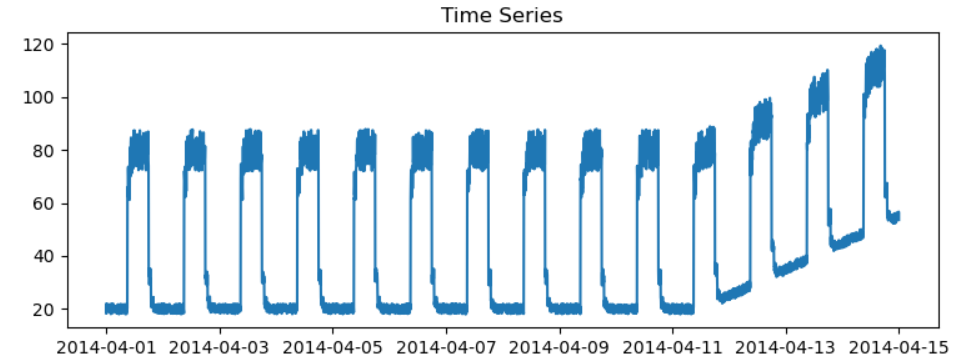
\includegraphics[width=10cm]{fig/numentaExample.PNG}
	\caption{Illustration einer Numenta-Zeitreihe\cite{AHMAD2017134}}
	\label{img:numentaTS}
\end{figure}


\section*{Netzwerk-Datens�tze}
\label{sec:netData}

Zwischen den Forschungsgruppen, welche sich mit der Ausrei�ererkennung in Netzwerken besch�ftigen, herrscht gro�e Konkurrenz. Aus diesem Grund werden gelabelte Datens�tze h�ufig zur�ckgehalten. Dadurch wollen die Forscher verhindern, dass sie ihren Wettbewerbsvorteil gegen�ber anderen verlieren \cite{Problematik}. Aus diesem Grund ist es schwer geeignete Datens�tze zu finden. Mit dem Enron- und Darpa-Datensatz konnten dennoch zwei passende Datens�tze ausgemacht werden. Diese Datens�tze werden im Folgenden vorgestellt.
 
\subsubsection{Enron}



Der Enron Datensatz enth�lt die intern versendeten E-Mail Daten von rund 150 Mitarbeitern der Firma Enron. Die Daten wurden von der Federal Energy Regulatory Commission offengelegt. Enthalten sind ca. 50.000 E-Mail-Nachrichten. F�r den Algorithmus wird lediglich der Zeitpunkt, an dem eine E-Mail versendet wird sowie die Sender und Empf�nger festgehalten.

F�r den Enron Datensatz stehen keine Labels zur Verf�gung. Aus diesem Grund wurden Ausrei�er, die der SedanSpot-Algorithmus gefunden hat, als Labels verwendet. \cite{SedanSpot}. Au�erdem vergleichen die Autoren des SedanSpot-Algorithmus ihre Ausrei�er mit der offiziellen Enron-Zeitleiste. Diese enth�lt ebenfalls Informationen �ber m�gliche historische Gr�nde f�r die Ausrei�er \cite{EnronTimeline}.


\subsubsection{DARPA}

Der DARPA-Datensatz \citep{DARPA} beinhaltet 4.5 Millionen IP-zu-IP-Kommunikationen zwischen 9.400 Quell-IP's und 23.300 Ziel-IP's �ber einen Zeitraum von 87.700 Minuten. Jede Kommunikation ist zu einem Zeitpunkt eine gerichtete Kante von der Quell-IP zur Ziel-IP. Eine vierte Spalte des Datensatzes ist verf�gbar, in der ein \textit{label} enthalten bzw. ein Angriff gekennzeichnet ist. Der DARPA-Datensatz besteht zu �ber 60\% aus Ausrei�ern. 
